\chapter{Attention Mechanism}
\section{Introduction}
In this section, we will focus on the deep learning models, the first one being a bidirectional LSTM and the second one an attention layer is added to this LSTM. But it is need to use an other text embedding in order to work with LSTM. Indeed, tf-idf create a sparse matrix with each row corresponding to a value for a given word. This means that the order of the words are lost. In order to solve this, word2vec\cite{Mikolov2013} is used. It allows to match words to continuous vectors of a given size with interesting properties. An other methods, which consist in making word embedding as tuning parameters will be used.

\section{Text to Vectors}
\subsection{Word2Vec}
Word2Vec comes in two fashions: continuous bag of word (CBOW) and skip-gram. It is originaly designed to predic a word given a context. For instance, given two previous words and the two next words, which word is the most likely to take place between them. But it appears that the hidden representation of these words works well as word embedding and have very interesing properties such that words with similar meaning have similar vector representation. It is also possible to perform arithmetic that captures informations such as singular, plural or even capital and countries. For example, we have that $dog - dogs \approx cat - cats$ but also $Paris - France \approx Berlin - Germany$. \\

It is possible to visualize these relasionships by using t-SNE for projecting high dimentions word vectors in 2D space. The results of various relashionships can be see at \textbf{Figure \ref{fig:chap4:word2vec}}.
\begin{figure*}
	\centering
	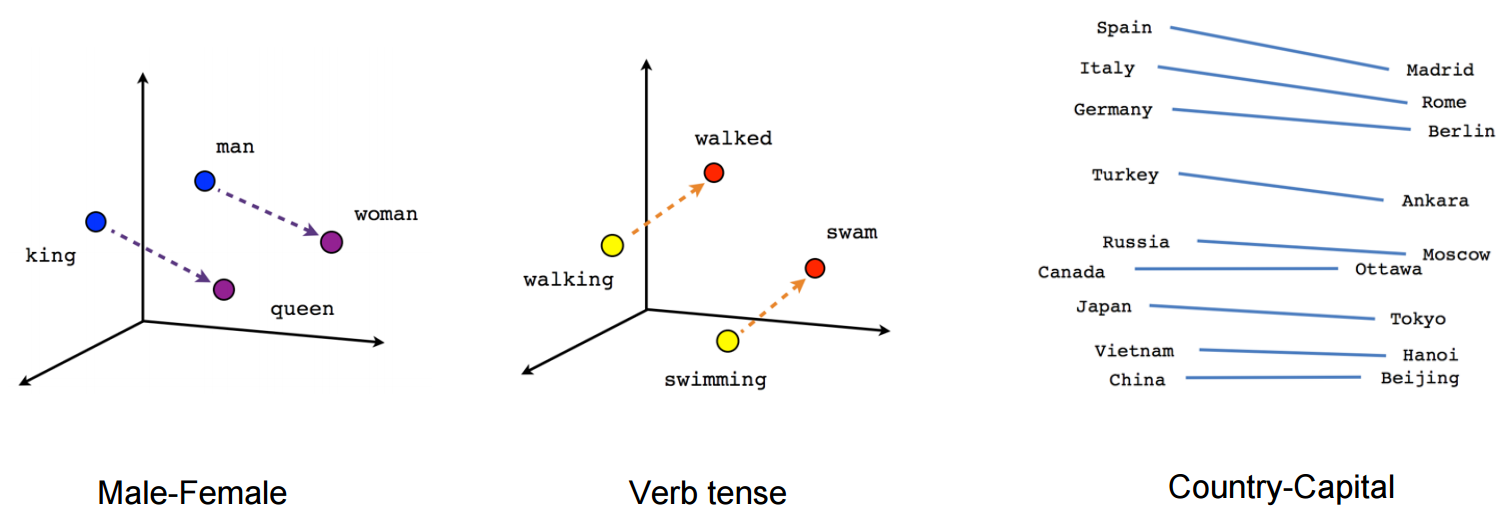
\includegraphics[width=\textwidth]{images/chapitre4/linear-relationships}
	\caption{Relashionships between different words with t-SNE dimentionality reduciton. }
	\label{fig:chap4:word2vec}
\end{figure*}

\subsubsection{How does it works?} 
As the orignal authors did not inteded this kind of results, Xin Rong\cite{Rong2014} did a good job explaing how it works. 

Let V be the size of the vocabulary and that there is only one word in the CBOW model, it give \textbf{Figure \ref{fig:chap4:CBOW}}. model. 

\begin{figure*}
	\centering
	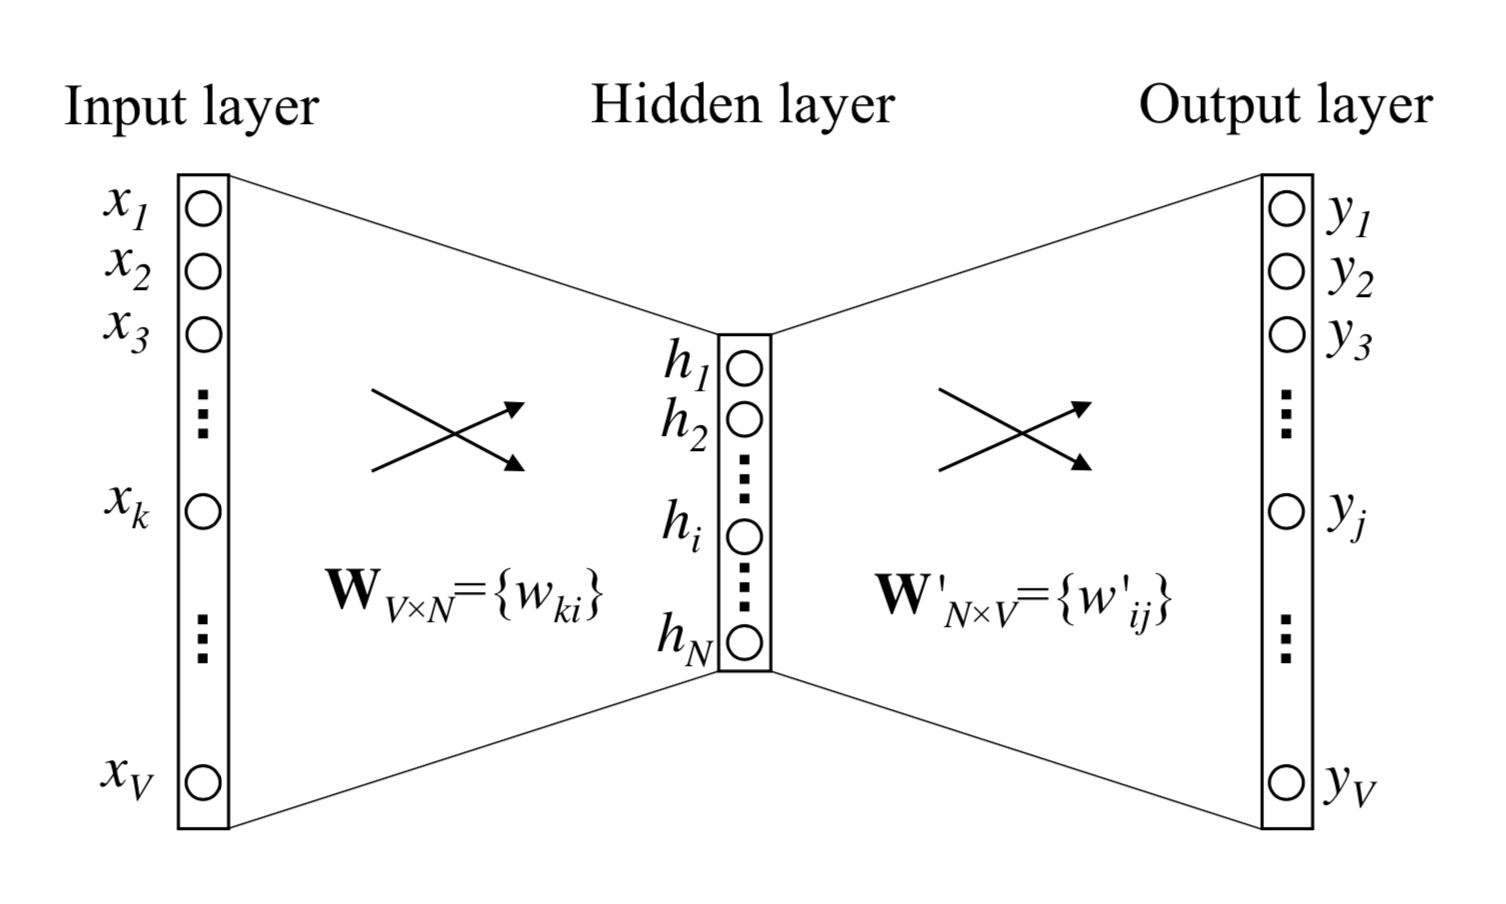
\includegraphics[width=\textwidth]{images/chapitre4/CBOW}
	\caption{A simple CBOW model with only one word in the context}
	\label{fig:chap4:CBOW}
\end{figure*}

\section{LSTM}
\section{Attention Mechanism}